\documentclass{style/ucasproposal}

\usepackage{style/commons}
\usepackage{style/custom}
\usepackage{pdfpages}
\usepackage[cache=false,outputdir=tmp]{minted}

\setmonofont{Fira Code}
\usemintedstyle{trac}
\newmintedfile[ccode]{c}{style=trac}
\newcommand{\cinline}[1]{\mintinline[style=trac]{c}{#1}}

\setcounter{tocdepth}{3}

\begin{document}

\pagenumbering{roman}

\includepdf[page={1}]{pages/fake-cover.pdf}

\tableofcontents

\clearpage
\pagenumbering{arabic}

% ---------------------------------
\section{题目描述和题目要求}
用 libgrahics 图形库及 simpleGUI ~\cite{simplegui} 编写一个俄罗斯方块游戏,实现

\begin{itemize}
    \item \textbf{基本功能}:移动、旋转和摆放输出的各种方块,并且在排列成完整的一行或多行时消除得分。
    \item \textbf{拓展功能}:难度等级、排行榜、存档读取/写入
    \item \textbf{特色功能}:原创或其他特色功能
\end{itemize}

用户体验上,要求简洁美观、可操作性好、执行速度快。

代码方面,要求在编写过程中代码规范、注释清楚,并运用链表的知识,采取多文件模块化组织结构。


% ---------------------------------
\section{需求分析}

以下是我们小组讨论得出的需求分析:

有关方块定义,我们需要能美观地绘制7种方块(分别为O型、I型、Z型、S型、J型、L型、T型),
这个过程包括\textbf{着色}以及\textbf{形状}的确定。

有关方块旋转及摆放,需实现\textbf{碰撞检测}功能,如考虑到用户体验,还要加入一个\textbf{到达边界不能旋转时,自
适应地作出水平位移以腾出旋转空间}的功能。

消除得分上,为增加挑战性,可采取\textbf{阶梯式得分制}:消除一行得到基准分,多行则有相应的加分。

难度等级,通过每消除一定行数时就\textbf{增加下落速度}来实现,但要有一个上限,比如最高5级,不能无限制提高难度。

排行榜,需要能展示前十位的玩家姓名及所得分数,从高到低排列;还要在一轮游戏结束时\textbf{提醒玩家保存分数记录}。

关于存档,我们需要能\textbf{保存/读取多个存档},根据用户名来组织。存档需要记录的东西有:
\begin{itemize}
    \item 已落下的方块堆(位置和颜色)
    \item 3个完整方块的坐标、方位和颜色(正在下落的、即将下落的、暂时储存的)
    \item 游戏数据:分数、难度等级、已消除行数
    \item 为保证完全恢复游戏进度的其他一些数据
\end{itemize}

有关特色功能,我们准备实现\textbf{方块暂存(\textit{hold})功能}、\textbf{交互式操作功能}。
\textbf{方块暂存},即将当前下落方块保存起来,并切换到下一个方块;在需要时,可将方块释出。该功能是为了平衡游戏难度,增加一点确定性。
\textbf{交互式操作},即在作出选择、操作成功/失败时使用对话框提醒用户,以及用对话框获取玩家输入等。



% ---------------------------------
\section{总体设计}
\subsection{功能模块设计}
\begin{itemize}
    \item \textbf{总体控制模块},负责用户事件捕捉和任务分配,以及界面显示刷新
    \item \textbf{方块操作模块},负责方块移动、旋转,以及碰撞检测、消除检测
    \item \textbf{流程控制模块},负责游戏数据、状态、进程控制
    \item \textbf{界面绘制模块},负责所有界面、菜单、窗口、方块的绘制
    \item \textbf{用户交互模块},负责各种交互式对话框的定义
    \item \textbf{文件处理模块},负责排行榜、游戏存档的存入/读取
\end{itemize}

\subsection{数据结构设计}

首先,作为基础,我们定义了一个坐标体系,用于方块的储存。其取值为整数,从 (0, 0) 到 (MaxCoordX, MaxCoordY) ,
即 (9, 20) ,并使用函数实现其与屏幕坐标系的互相转换。

在此基础上,对于最核心的数据结构——方块,我们设计了两种方案:\textbf{链表表示法}和\textbf{相对表示法},现具体分析两种方案:

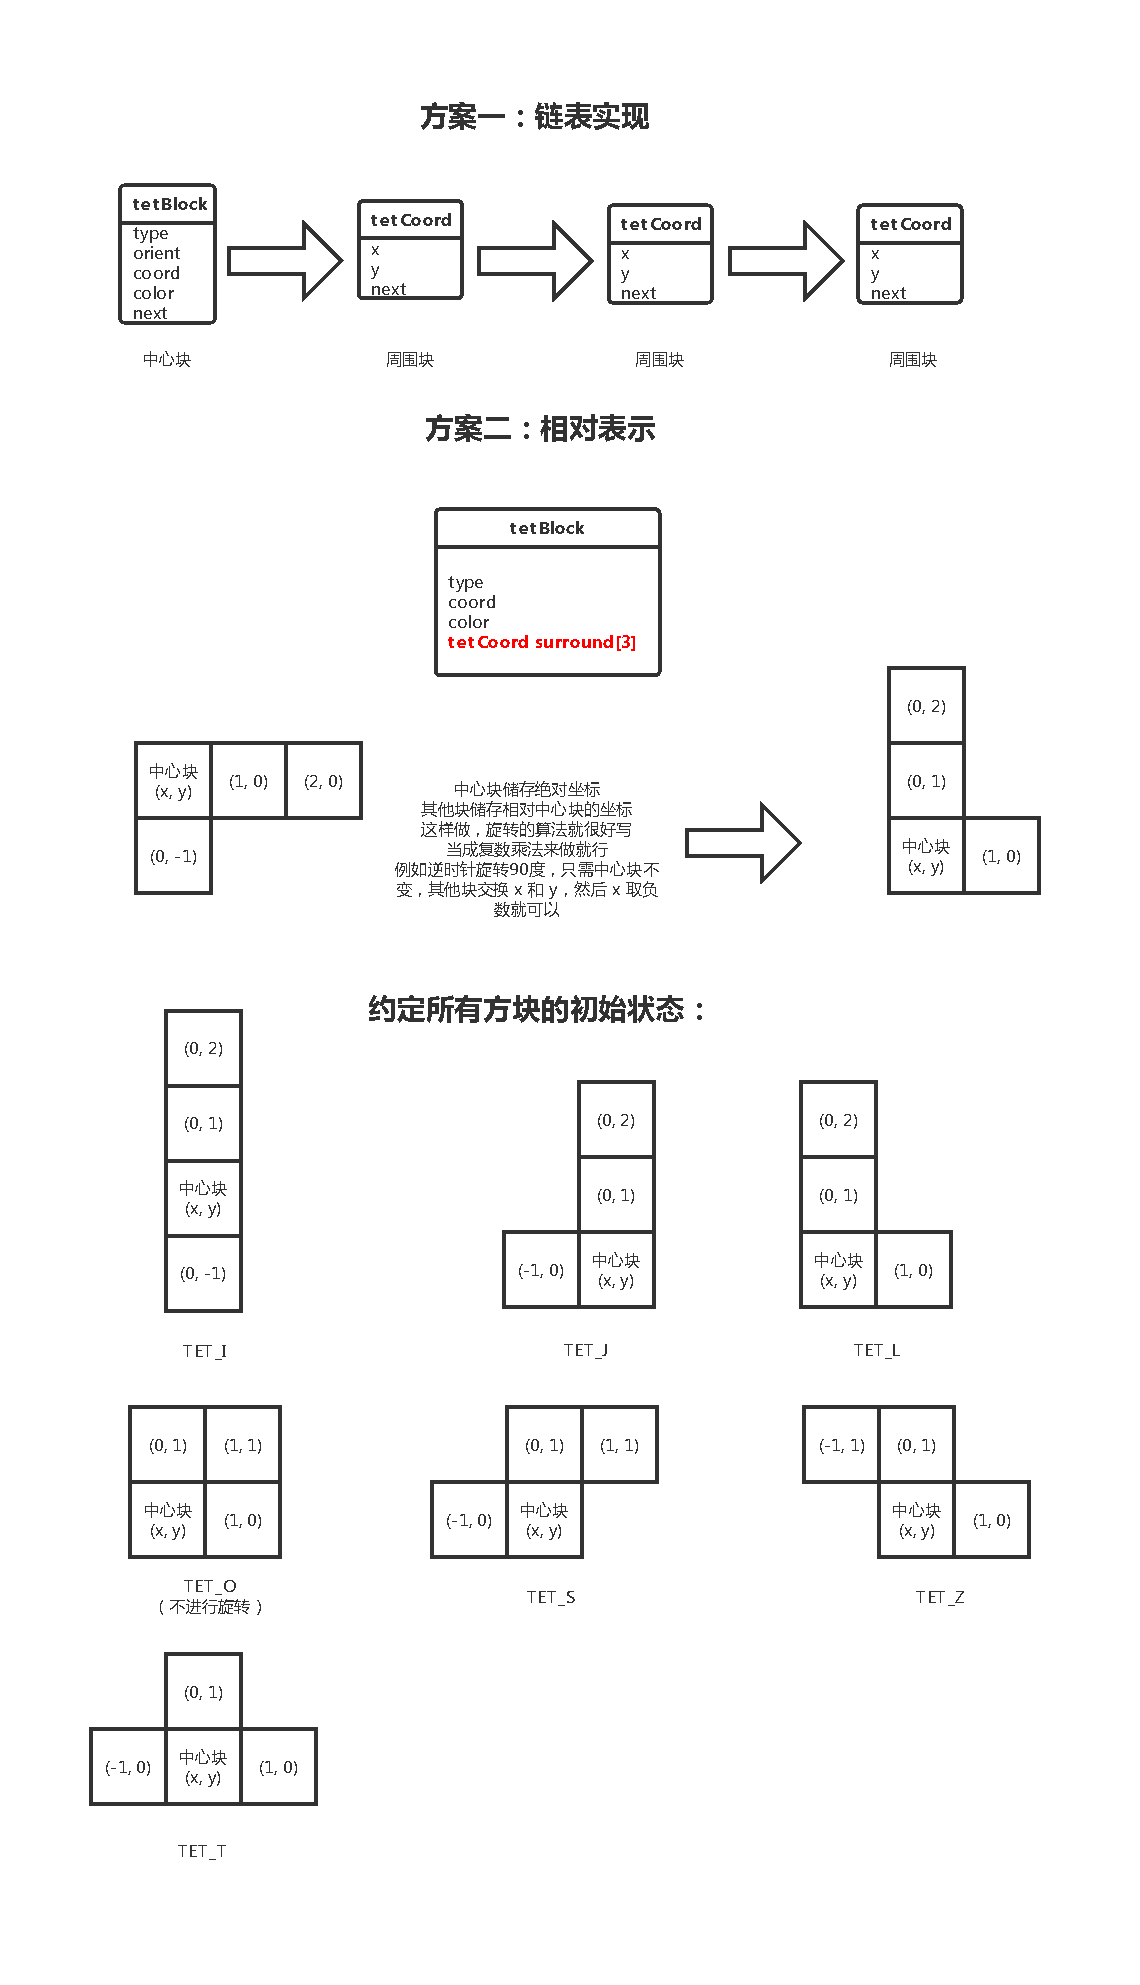
\includepdf[page={1},offset=0 -2cm]{pages/tetris.pdf}

1. 链表表示法。需定义4个节点(每个节点代表一格),包含类型、坐标、颜色、方位四个信息。除了坐标之外,其他3个信息只需储存一次。
因此定义两种结构,一种是头结点 \cinline{tetBlock} ,含有方块的完整信息;另一种是 \cinline{tetCoord} ,储存周围3个块的坐标。


2. 相对表示法。实际上,该方案与第一种链表法本质等价,因为链表中的周围块坐标减去中心坐标就得到相对坐标。
但因为它把信息都压缩到了一个结构里,相比链表表示有着\textbf{节省空间}、\textbf{操作简单}(无需考虑当前方向,移动只需改变一个方格,即中心格坐标,旋转只需做一个复数乘法)、\textbf{容易储存}(信息在内存中连续)的优点,因此我们最终选用了相对表示法作为方块的结构。
(事实上后来在助教提示下我们想到了更好的用链表来表达的方案,但时间已经不允许重构了)
\newline

对于已落下的方块堆,我们定义了一种以单格为单位的数组结构,包含占用信息和颜色信息:
\begin{minted}{c}
typedef struct {
  tetCellStatu statu;
  tetColor color;
} tetBoard;
\end{minted}
其中, \cinline{tetCellStatu} 是一个枚举类型,表示当前格是否已被占用,有 \cinline{CELL_EMPTY}
 和 \cinline{CELL_TAKEN} 两种取值;
\cinline{tetColor} 则是一种表示颜色的枚举类型。有关坐标如何体现,我们采取二维数组来定义:
\cinline{tetBoard stored[/*rows*/][/*cols*/]},
主要是因为其有着\textbf{在内存中连续储存}的优点,极大地方便代码编写和效率优化。
例如,清空方块堆只需一次库函数调用:

\cinline{memset(&stored[0][0], CELL_EMPTY, sizeof(stored));}

在消除一行时,我们也可以简单地使用 \cinline{memcpy} ~\cite{tinytetris} 函数来做到;
同理,在存档时,也可直接使用一次 \cinline{fwrite} ~\cite{fwrite} 来保存整个方块堆。
\newline

对于分数记录,我们使用链表的形式储存,由文件处理模块中的 \cinline{loadRecords} 和 \cinline{saveRecord} 进行统一管理,
存放在 \cinline{saves/records} 文件中。
\begin{minted}{c}
typedef struct tetRecord tetRecord;
struct tetRecord
{
  char       name[NAMELEN]; // 用户名
  int        score; // 分数
  tetRecord* next;
};
\end{minted}


游戏存档则储存在 \cinline{saves/} 目录下,通过用户名进行组织,文件名为\newline
\mintinline[style=trac]{perl}{${username}.save} 。
其文件结构采取\textbf{二进制形式},直接dump内存中表示方块堆和各方块的区域,以及一些游戏状态变量。


\subsection{重要函数功能描述}

概览:(可点击跳转)
\begin{itemize}
    \item \hyperref[func:collisionCheck]{collisionCheck -> 碰撞检测}
    \item \hyperref[func:eliminateLines]{eliminateLines -> 高效的方块消除函数}
    \item \hyperref[func:rotate]{rotate -> 自适应的方块旋转函数}
    \item \hyperref[func:MsgBox]{MsgBox -> 通用交互式对话框框架}
    \item \hyperref[func:loadGame]{loadGame -> 带exception处理的存档读取函数}
\end{itemize}

\subsubsection{collisionCheck -> 碰撞检测}
\label{func:collisionCheck}
\begin{minted}{c}
tetBoundStatu collisionCheck()
/* 函数名称:collisionCheck
 * 函数原型:tetBoundStatu collisionCheck()
 * 功能描述:对正在下落的方块进行碰撞检测
 * 引起效果:无
 * 参数描述:无
 * 重要局部变量:无
 * 返回类型:tetBoundStatu,表示方块碰撞检测结果
 *        (枚举类型tetBoundStatu定义见方块处理模块tetris.h)
 * 可能取值:
 *      FREEMOVE    - 未碰撞
 *      COLLIDED    - 与堆中方块或界面底部碰撞
 *      LEFT_BOUND  - 与左边界碰撞
 *      RIGHT_BOUND - 与右边界碰撞
 *
 * 注:在多种状态同时成立时,比如,同时与方块堆和左边界碰撞
 *    优先返回左右边界值,这是为了方便在边界上旋转时的自适应功能
 * --------------
 * 函数算法描述:
 *      算法开始
 *   -> 分别对中心格和3个周围格做检查
 *      -> 是否超出左右下边界(不检查上边界,因为方块会从上方生成)
 *      -> 当前格是否已被占用
 */
\end{minted}

\subsubsection{eliminateLines -> 高效的方块消除函数}
\label{func:eliminateLines}
\begin{minted}{c}
int eliminateLines()
/* 函数名称:eliminateLines
 * 函数原型:int eliminateLines()
 * 功能描述:消除检测,并作出处理
 * 引起效果:改变全局变量stored
 * 参数描述:无
 * 返回类型:int,表示消除的行数
 * 重要局部变量:
 *  tetBoard* curp  -> 指向当前处理的格子
 *  bool lineFilled -> 指示当前行是否已满
 * --------------
 * 函数算法描述:
 *      算法开始
 *   -> 从上到下,按行扫描
 *   -> 如当前行已满
 *       -> 将上一行的连续内存拷贝到当前行
 *       -> 消除行+1
 *       -> 对上面的所有行作出该操作
 *   -> 返回消除行数
 */
\end{minted}

\subsubsection{rotate -> 自适应的方块旋转函数}
\label{func:rotate}
\begin{minted}{c}
void rotate()
/* 函数名称:rotate
 * 函数原型:void rotate()
 * 功能描述:顺时针旋转正在下落的方块
 * 引起效果:改变全局变量falling
 * 参数描述:无
 * 返回类型:无
 * 重要局部变量:无
 * --------------
 * 函数算法描述:
 *      算法开始
 *   -> 对O型方块,直接返回,无需旋转;
 *   -> 中心格不变,对周围格进行复数乘法,即交换 x 和 y,再对 y 取负
 *   -> 调用碰撞检测函数进行检测
 *      -> 如通过,则返回
 *      -> 如与左右边界碰撞
 *          -> 进行水平位移以适应,返回
 *          -> 如无法适应,则恢复原状态,返回
 *      -> 如与底部或方块堆碰撞,则恢复原状态,返回
 */
\end{minted}

\subsubsection{MsgBox -> 通用交互式对话框框架}
\label{func:MsgBox}
\begin{minted}{c}
int MsgBox(char* prompt, char* buttons[], int n,
            int hasTextBox, char* strBuffer, int buflen);
/* 函数名称:MsgBox
 * 函数原型:int MsgBox(char* prompt, char* buttons[], int n,
                    int hasTextBox, char* strBuffer, int buflen);
 * 功能描述:显示一个立体效果的、宽度自适应的交互式对话框,有文本框输入功能(可选)
 * 引起效果:界面绘制
 *
 * 参数描述:
 *   prompt :: char*     - 提示消息
 *   buttons[] :: char*  - 按钮列表
 *   n :: int            - 按钮个数
 *   hasTextBox :: int   - 是否含有文本框(0-否 1-是)
 *   strBuffer :: char*  - 文本框的输入缓冲区(如果不用文本框请设为NULL)
 *   buflen :: int       - 文本框缓冲区大小(不用文本框请设为0)
 *
 * 返回类型:int
 *   -1    - 用户没有点击(按下并释放)按钮
 *   >=0   - 用户点击的按钮 index (在buttons[]中)
 *
 * 重要局部变量:
 *  double widthOfButtons, widthOfPrompts
 *        -> 分别表示按钮和提示文字需占用的宽度,其较大者决定对话框宽度
 *
 *  int k -> 在循环绘制所有按钮的过程中暂存按钮按下状态
 * --------------
 * 函数算法描述:
 *      算法开始
 *   -> 根据提示文字长度及按钮个数计算边框宽度、内容排版位置
 *   -> 绘制内外方框(立体阴影效果)
 *   -> 绘制提示文字
 *   -> 如果有文本框,则绘制
 *   -> 循环绘制所有按钮,并记录按下状态
 *   -> 返回按钮按下结果
 */
\end{minted}

\subsubsection{loadGame -> 带exception处理的存档读取函数}
\label{func:loadGame}
\begin{minted}{c}
int loadGame(char* username)
/* 函数名称:loadGame
 * 函数原型:int loadGame(char* username)
 * 功能描述:读取一个玩家的游戏存档,自带错误处理
 *         | 存档目录为 saves/
 *         | 文件名为 $(username).save
 * 引起效果:引起磁盘读取、引起游戏状态及数据的改变
 * 参数描述:玩家名 name :: char*
 * 返回类型:int,代表读取结果
 *         成功       返回 SUCCESS
 *         读取失败    返回 FAILURE
 * 重要局部变量:exception InvalidFormat -> 代表存档格式错误
 * --------------
 * 函数算法描述:
 *      算法开始
 *   -> 根据传入用户名参数,打开对应存档文件
 *      -> 文件不存在或打开失败
 *           -> 返回 FAILURE
 *      -> 文件打开成功
 *      -> 进入 try 块
 *      -> 使用自定义的安全读取宏 SafeRead 读取记录
 *           -> 中间发生任何错误
 *           -> 转向 except,返回 FAILURE
 *      -> 读取完成,返回 SUCCESS
 */
\end{minted}


\subsection{程序文件结构}
\subsubsection{文件函数结构}

共6个C代码文件,5个头文件:

\begin{itemize}
    \item \textbf{总体控制模块}(main.c)     - 用户事件捕捉和任务分配,以及界面显示刷新
    \item \textbf{方块操作模块}(tetris.c)   - 方块移动、旋转,以及碰撞检测、消除检测
    \item \textbf{流程控制模块}(flow.c)     - 游戏数据、状态、进程控制
    \item \textbf{界面绘制模块}(layout.c)   - 所有界面、菜单、窗口、方块的绘制
    \item \textbf{用户交互模块}(interact.c) - 包含一个通用的交互式对话框框架,以及各种交互式对话框的定义
    \item \textbf{文件处理模块}(fileIO.c)   - 排行榜、游戏存档的存入/读取
\end{itemize}

$\lambda$\newline
\textbf{总体控制模块}(main.c) 包含函数有:\newline
程序入口点:\cinline{Main}\newline
用户事件捕捉:\cinline{CharEventProcess}, \cinline{MouseEventProcess}, \cinline{KeyboardEventProcess}\newline
界面刷新:\cinline{SetBackground}, \cinline{display}

$\lambda$\newline
\textbf{方块操作模块}(tetris.c) 包含函数有:\newline
方块形态控制:\cinline{initBlock}, \cinline{rotate}\newline
方块位置控制:\cinline{move}, \cinline{drop}, \cinline{moveToTop}, \cinline{moveToNextBox}, \cinline{moveToHoldBox}\newline
方块堆操作:\cinline{addToBoard}\newline
方块生成与检测:\cinline{geneNext}, \cinline{collisionCheck}, \cinline{eliminateLines}\newline
其对应的\textbf{头文件(tetris.h)} 主要包含方块结构、外观、位置、运动相关的定义

$\lambda$\newline
\textbf{流程控制模块}(flow.c) 包含函数有:\newline
游戏初始化(控制与数据):\cinline{initTetris}, \cinline{initGameData}\newline
计时器回调函数:\cinline{TimerFallingEvent}\newline
游戏状态控制:\cinline{setGameStatu}, \cinline{getGameStatu},\newline
\cinline{getPrevStatu}, \cinline{restoreGameStatu}, \cinline{isOnHolding}\newline
游戏进程控制:\cinline{gameStart}, \cinline{gamePause}, \cinline{gameResume}, \cinline{gameOver},\newline
\cinline{levelUp},\cinline{hold}, \cinline{newRound}\newline
游戏数据控制:\cinline{addScore}, \cinline{getScore}, \cinline{getLevel}, \cinline{getLines}\newline
其对应的\textbf{头文件(flow.h)} 主要包含游戏状态、流程及相关操作接口的定义

$\lambda$\newline
\textbf{界面绘制模块}(layout.c) 包含函数有:\newline
游戏界面绘制:\cinline{dispFrame}, \cinline{dispStat}\newline
游戏菜单、标题栏绘制:\cinline{dispGameMenu}, \cinline{dispHeader}\newline
游戏各窗口绘制:\cinline{dispStartWindow}, \cinline{dispRankWindow}, \cinline{dispHelpWindow}\newline
坐标操作:\cinline{coordToInch}\newline
方块绘制:\cinline{fillCell}, \cinline{drawBlock}, \cinline{dispStored}, \cinline{dispFalling},\newline
\cinline{dispNext}, \cinline{dispHold}, \cinline{dispAllBlocks}
其对应的\textbf{头文件(layout.h)} 主要包含界面位置、大小相关的数据和外部接口定义

$\lambda$\newline
\textbf{用户交互模块}(interact.c) 包含函数有:\newline
通用的交互式对话框框架:\cinline{MsgBox}\newline
各种交互式对话框的定义:\cinline{MsgBoxResume}, \cinline{MsgBoxSave},\newline
\cinline{MsgBoxLoad}, \cinline{MsgBoxSuccess}, \cinline{MsgBoxLoadFail},\newline
\cinline{MsgBoxSaveFail}, \cinline{MsgBoxRestart}, \cinline{MsgBoxBackToMain},\newline
\cinline{MsgBoxGameOver}, \cinline{MsgBoxRecord}
其对应的\textbf{头文件(interact.h)} 主要包含通用交互式对话框框架及各种对话框的声明

$\lambda$\newline
\textbf{文件处理模块}(fileIO.c) 包含函数有:\newline
链表处理:\cinline{freeRecords}\newline
排行榜存取:\cinline{loadRecords}, \cinline{saveRecord}\newline
游戏存档存取:\cinline{loadGame}, \cinline{saveGame}\newline
其对应的\textbf{头文件(fileIO.h)} 主要包含分数记录链表数据结构定义和IO接口的声明

\subsubsection{多文件构成机制}
我们将函数根据功能进行了严格的分类,归到其所属模块下。同时,对于数据结构、各种宏与常量,我们也进行了细致的分类,做到头文件内容的最小化,只在本模块用到的东西就一定不让其导出。同时,我们逐一地确定了头文件的包含关系,确保每一个\#include指令都是必要的。
我们自己编写的每个头文件,在被包含时都加上了注释,注明包含的原因,以便功能调试和拓展。

有关\#define保护,我们为每一个头文件都定义了宏名,将整个头文件内容放进
\mintinline[style=trac]{c}{#ifndef...#define...#endif}结构中,
保证了头文件只被包含一次。

外部变量我们进行了严格控制,用得很少,主要就是\textbf{流程控制模块}中定义的游戏数据需要在\textbf{文件处理模块}中可见,以进行存档的读入与保存;以及与界面绘制相关的模块都引入了主函数模块中的 \cinline{winwidth, winheight}。
实际上我们可以完全不用任何外部变量,而通过\textbf{为函数加上指针参数}来进行操作,但我们用到的这些外部变量在游戏过程中都只有\textbf{唯一实例},因此没有必要进一步抽象化。



% ---------------------------------
\section{部署与运行}
\subsection{编译安装运行说明}
源代码目录结构应如图所示:
\begin{minted}{shell}
tetris/
├── lib/
│   ├── libgraphics/
│   └── simpleGUI/
├── project/
│   └── dev-cpp/
├── report/
├── Makefile
├── main.c
├── fileIO.c
├── fileIO.h
├── flow.c
├── flow.h
├── interact.c
├── interact.h
├── layout.c
├── layout.h
├── tetris.c
└── tetris.h
\end{minted}

编译方式:
\begin{itemize}
    \item 方法一:直接打开project/dev-cpp/下的工程文件进行编译
    \item 方法二:如果dev-cpp安装在默认目录,且 GCC 在 PATH 环境变量中,可直接在当前目录执行 make 命令编译
\end{itemize}

编译结果应在当前目录下得到一个 tetris.exe 文件。

\textbf{有关程序使用,请参考用户使用手册 manual.pdf}

\subsection{典型测试情况}

\subsubsection{旋转算法对碰撞检测先后顺序的依赖}

在调试方块旋转的自适应功能时,我们发现在\textbf{极端情况}下(中央方块几乎堆积到顶,两边空间狭窄)
旋转方块会引起程序陷入死循环,当时我们旋转算法对边界碰撞的处理是这样的:\textit{如与左右边界碰撞,则向相反方向作出水平位移,直到\textbf{不引起冲突}}。

仔细分析后,我们发现了其中的原因:这种逻辑在两边空间空旷时是有效的,但对于上述极端情况,几乎每一步水平位移都会引起冲突,导致方块一直作出位移,\textbf{从另一侧超出了游戏区域},
此时我们的碰撞检测函数会给出与另一边界碰撞的结论,从而导致方块折返。
因此方块就不断在左右边界来回运动,陷入死循环。

针对该问题,我们改进了算法:\textit{如与左右边界碰撞,则向相反方向作出水平位移,直到\textbf{不与该边界碰撞}时停止移动,且此时不与已有方块堆发生冲突才能旋转}。

改进后的算法顺利通过了上述极端测试,但更进一步的测试又暴露了\textbf{新的问题}:在下落方块同时贴近方块堆与左右边界时,进行旋转,
可能导致方块“嵌入”到已有方块堆中。

该bug比较隐蔽,我们在小组讨论中未找出其原因。后来在整理碰撞检测函数代码的过程中,发现这是由于未考虑到多种可能结果的原因:
我们需要处理方块同时与左右边界和方块堆冲突的情况,而我们现有的碰撞检测逻辑在此种状态下得出的结果是:返回代表与方块堆冲突的值,而忽略了边界情况。

对此,我们提出了\textbf{两种方案}:专门分配一个值来表示这种情况,或提高边界检测的优先级。
由于两种方案都能得出有效结果,因此虽然第一种方案更加全面,但我们采取了效率比较高的第二种方案。
同时我们也在头文件tetris.h中声明碰撞检测函数的地方特意注明了此种边界情况,以供功能扩展时参考。


\subsubsection{对 simpleGUI 的两个改进}

(1)在调试文本框输入时,我们发现,当输入长度达到缓冲区限制后,继续按下一个字符,再按下退格键,此时文本框中最后一个字符并没有得到删除,
而是被替换为了刚才按下的字符。
经过对imgui.c中textbox函数代码的分析,我们认为这是由于 \cinline{gs_UIState.charInput} 在按下退格键后并没有被置零,导致刷新界面时将该字符当成输入而导致的,因此我们对imgui.c作出修改,检测到退格键就把输入暂存变量置零:

\begin{minted}{diff}
--- /run/shm/code/tetris/lib/simpleGUI/imgui(old).c
+++ /run/shm/code/tetris/lib/simpleGUI/imgui.c
@@ -540,6 +540,7 @@
            gs_UIState.keyPress = 0;
            break;
        case VK_BACK:
+           gs_UIState.charInput = 0;
            if( len > 0 ) {
                textbuf[--len] = 0;
                textChanged = 1;
\end{minted}

改进后的版本解决了这一问题。

(2)另外,在开发的早期,我们就注意到了一个问题:最后绘制的一个控件(button或menu)在鼠标移上去时会“干扰”周围其它线条的颜色,
不过当时有更要紧的功能需要实现,并没有深入研究。在项目即将完成时,我们才将这一问题重新提上议程。

我们写了一些测试程序,画了很多控件,试图找到规律。最终发现:受到干扰的控件都是在该按钮之后绘制的,因此我们猜想,是由于button函数
在设置自身的热点颜色后,未将颜色复原导致的,因此我们改进了button函数,在颜色修改之前保存上一个颜色,返回前将其恢复:

\begin{minted}{diff}
--- /run/shm/code/tetris/lib/simpleGUI/imgui(old).c
+++ /run/shm/code/tetris/lib/simpleGUI/imgui.c
@@ -259,6 +259,7 @@
 {
    char * frameColor = gs_button_color.frame;
    char * labelColor = gs_button_color.label;
+   char * prevColor  = GetPenColor();
    double movement = 0.2*h;
    double shrink = 0.15*h;
    double sinkx = 0, sinky = 0;
@@ -316,9 +317,11 @@
    {
        gs_UIState.clickedItem = 0;
        gs_UIState.kbdItem = id;
+       mySetPenColor(prevColor);
        return 1;
    }

+   mySetPenColor(prevColor);
    return 0;
 }
\end{minted}

实际上,这一问题仅仅是简单的\textbf{抽象泄漏},并不算严重的bug,只要我们在绘制自己的控件前都设置一遍颜色,就不会出现任何问题。


% ---------------------------------
\section{组内分工}
\subsection{组内分工及参与度}
\begin{tabular}{cccc}
\hline
姓名  &     HSL    &     RFJ     &       YXN        \\
参与度 &     9      &       9     &       10           \\
\hline
分工  &  方块显示    &  方块消除检测 & 模块架构、数据结构设计 \\
     & 排行榜界面设计 & 帮助界面设计  & Hold功能、交互系统设计\\
     &   代码整理    &  分数记录读取 & 程序报告与用户手册撰写 \\
     &    debug     &             & 代码规范、重构与优化  \\
\hline
\end{tabular}
\subsection{实践中遇到的难点及解决方案}
\subsubsection{HSL}
我在实践当中遇到的最大的一个难点就是,要\textbf{如何显示俄罗斯方块的各种形状。}
因为表示的方法是多种多样的,可以用一个二维数组,也可以采用链表的形式,因此也重复写了很多次代码。

最后为了使控制俄罗斯方块的代码易于编写,
经过小组商讨后,我们决定构建一个“中心块+周围块相对中心块坐标”的结构体来表示每一个方块
(这样在俄罗斯方块移动时,周围块的坐标可以不动,只需要改动中心块的坐标即可)。

\subsubsection{RFJ}
我在实践中遇到了多个难点。

一是\textbf{对编写绘图程序不够熟悉,}不知道怎么正确使用。
比如不熟悉把按钮、文本框和数据运算联系起来,于是照着PPT将示例程序作尝试性的修改,并把学到的东西应用在俄罗斯方块中;
比如记不清可以调用的函数有哪些,为此把所有函数按照自己的方式又整理并试验了一遍。

二是\textbf{对程序的组织方式不明白,}写了模块却不知道怎么和整体程序组织起来。
在团队的帮助下知道了是要对Makefile文件进行修改,在队友帮忙修改Makefile文件的过程中,也对Makefile文件有了一点点了解。

三是\textbf{对用Git进行协同编程的方法不清楚。}这也是在队友的帮助下,了解到了如何上传代码、同步代码等等。


\subsubsection{YXN}

一是\textbf{“返回”、“取消”功能的编写}。在我负责的交互式对话框系统中,有很多对话框都有一个“取消”按钮,
其功能并不简单。比如帮助界面的“返回”按钮,就需要根据上一个游戏状态来决定按下按钮的行为,
因为用户可以在游戏主界面或者游戏过程中点击进入帮助页面,
对于从主界面进入的情况,按下返回按钮应该回到主界面;
而对于在游戏过程中进入帮助界面的情况,就需要返回游戏暂停的状态。

解决方案:重写流程控制模块flow.c里设置游戏状态的函数,使其在每一次改变状态时都保存上一个状态;
以及增加两个处理上一状态的外部接口。

二是\textbf{需要随时掌握整个工程的架构,}在新功能没有正常工作时,需要快速定位修改位置。
为此,我紧跟每一次代码提交,画了很多\textbf{思维导图、UML图}来组织模块与数据结构。

三是\textbf{处理模块间的依赖关系}。原先工程只分了3个模块,功能划分较不明确,随着功能的增多而越来越臃肿,
因此我花了一定时间\textbf{进行重新架构},降低了模块间的耦合度,确保了每个头文件包含都是必要的。

但仍有\textbf{未解决的问题},
就是流程控制模块flow.c、方块操作模块tetris.c、文件处理模块fileIO.c都包含了与界面绘制有关的头文件layout.h,
但这三个模块仅仅是为了使用其中的两个表示下落方块堆长和宽的宏定义,
我努力了很久,也没找到方法消除这个十分不必要的耦合,在各个模块中分别声明这两个宏当然是不可取的方法。
\textbf{后经助教提醒},我才意识到这就是\textbf{二维数组相对于链表表示的缺陷,}
因为数组中每一个内存单元都是用来储存有效信息的,没有多余单元能用来指示边界,所以这层依赖无法去除。
但重构已经来不及了,要重写的代码太多,大量注释、文档也要修改,因此只好保留这层依赖。
但我仍然感谢助教,与他的交流使我更清楚地认识到了二维数组与链表结构各自的优劣,以及自身考虑的欠缺。


% ---------------------------------
\section{合作纪要}
\begin{center}
\begin{figure}[H]
\center
    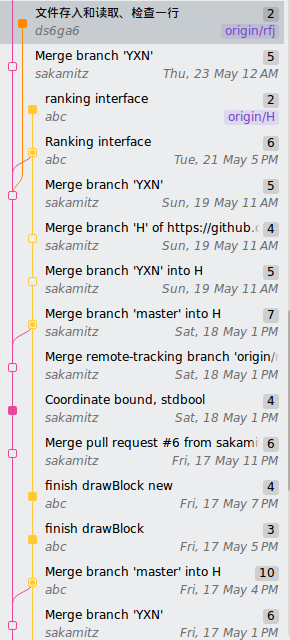
\includegraphics[width=0.6\textwidth]{./img//collaboration/tree.png}
\end{figure}
Git提交树(截图于5月24日)

(另有4张微信讨论长截图,不过被加密了)
\end{center}

% ---------------------------------
\section{总结}
\subsection{程序亮点与创新之处}
\subsubsection{Hold功能}
Hold功能,即玩家可以将当前下落方块暂存,流程切换到下一个方块;
在需要时,玩家可以将暂存的一个方块释放(\textit{release})出来代替当前方块,当前方块则被延迟一轮。

Hold功能可以丰富游戏内容,调节游戏平衡度,为完全随机的俄罗斯方块游戏\textbf{引入一点确定性}。

\subsubsection{交互式系统}
我们实现了 GUI 程序通常有的对话框机制,
游戏中的每一个会引起流程变化的操作都会有相应的操作提示,如下图:

\begin{center}

\begin{figure}[H]
\center
    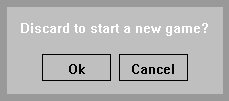
\includegraphics[height=0.15\textheight]{./img/restart.png}
\end{figure}
重新开始

\begin{figure}[H]
\center
    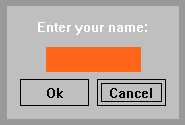
\includegraphics[height=0.18\textheight]{./img/name-input.png}
\end{figure}
输入名字

\begin{figure}[H]
\center
    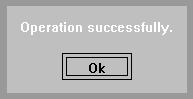
\includegraphics[height=0.15\textheight]{./img/success.png}
\end{figure}
读取存档成功

\begin{figure}[H]
\center
    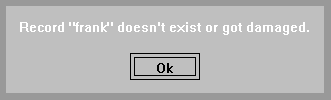
\includegraphics[height=0.15\textheight]{./img/failure.png}
\end{figure}
读取存档失败
\end{center}

\subsubsection{多个存档的支持}
游戏支持多个存档,按用户名进行组织,存放在 \cinline{saves/} 目录下,文件名为 “用户名” + \cinline{.save}

存档能\textbf{完全恢复游戏状态},包括方块堆、正在下落的方块、下一个方块、暂存的方块,以及 hold 状态、分数、难度等级等数据。

\subsubsection{游戏流程设计严密}
游戏一共有14个状态,但在这么繁多的状态间切换,并不会引发问题,这得益于模块化的设计,便于总控模块进行任务调度。

\subsubsection{界面美观易用}
\begin{center}
\begin{figure}[H]
\center
    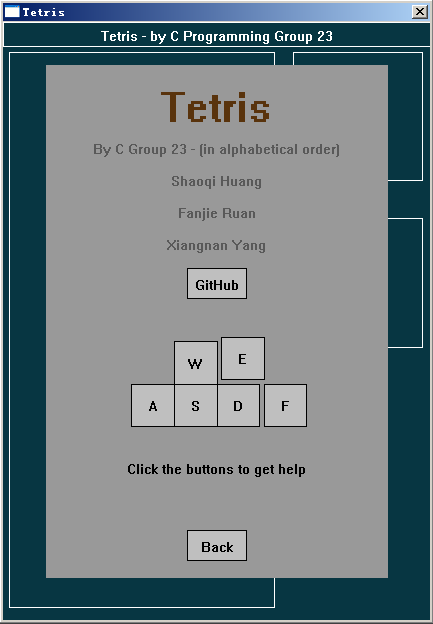
\includegraphics[width=0.7\textwidth]{./img/help.png}
\end{figure}
帮助界面,按下按钮会有提示
\end{center}

\textbf{有关程序使用,请参考用户使用手册 manual.pdf}

\subsection{应用知识点}
\begin{itemize}
    \item \textbf{链表的建立与操作}:我们使用链表来组织分数记录数据,在此过程中
    更加熟悉了链表的遍历和释放,以及节点的插入和删除。
    \item \textbf{文件的创建与存取}:在文件处理模块fileIO.c中,我们处理了文本文件、
    二进制文件的读取与写入,熟悉了文件的各种操作模式,以及fscanf、fprintf等函数的使用。
    \item \textbf{二维数组及指针的操作}:在方块消除与检测中,我们使用指针来遍历二维数组;
    同时存档采取二进制存取的方式,也让我们对数组的内存表示有了更深刻的认识。
    \item \textbf{头文件的组织与使用}:在编写模块化程序的过程中,我们对头文件的作用、
    机制,以及头文件保护方式有了更多的了解。
    \item \textbf{图形界面程序的编写}:相对于命令行程序,图形界面程序采取事件回调的方式运行。
    在利用 simpleGUI 提供的控件编写程序的过程中,我们深入认识到了图形界面的运行流程与机理。
\end{itemize}


\subsection{心得体会}
\textbf{良好的分工合作与交流十分重要}。一方面,在我们的相互协调中,程序的框架一点点的搭建了起来、内容一点点的丰富了起来。通过分享想法、沟通合作,三人合作编写程序的速度、效率远比一个人要高得多,也有趣得多。遇到困难后,团队一起解决也能有更多的想法。另一方面,在团队合作的相互分享中,我们也了解到了别人的想法,学习到了别人的经验。

\textbf{注意规范与协调}。比如外部接口,其作用与行为一定要说明清楚,便于他人正确地进行调用,
以及顺利合并各成员的编码进度。

\textbf{及时交流与跟进}。有时候其他成员编写的进度比较快,出现了许多更新更好的思路,
而如果没有注意代码的编写进度,仍旧按照最初的方式来编写自己负责的部分,
就会导致各个部分代码的不协调,需要重新花费功夫编写,加大了工作量;
同时,进度较快的成员也应及时告知团队相关的更改,并清楚明白地注释自己增加的部分。

\subsection{自我评价}
\subsubsection{HSL}
由于我本人的编程能力较弱,在整个团队设计大程序的过程中,出到的力是最小的。
我仅仅完成了俄罗斯方块的显示部分以及排行榜页面的设计部分,还有一些调试的任务。
因此我十分感谢其他两位同学,是他们承担了大部分的工作。

但是,在整个代码编写的过程中,我认为属于我自己的部分,我还是\textbf{能够尽职尽责地完成}。
尽管有时候为了弄懂一个原理,我需要上网查询大量地资料,不断重复看老师提供的课件,有时候在电脑前一坐就是五六个小时,但是我还是坚持了下来,并且在整个过程中,我认为自己的水平有了一定的提高。

而在整个团队的合作过程中,我所承担的更多是一个“接受任务者”的角色,在编程思路方面,比较少能够提出一些建设性意见。
但是在整个游戏的设计与制作灵感方面,我认为自己还是\textbf{提出了一些比较不错的意见},也算是对团队有所贡献。

\subsubsection{RFJ}
在这一次的团队设计中,我主要还是承担着一个接受任务、然后再解决任务的角色。
对整体框架的构思并没有太多的贡献,除了几次讨论。
但是我也\textbf{努力尽快、尽好地解决分到我这儿的任务,}并且在当前任务解决后,时间也比较空闲的情况下去询问有没有还需要做的。
又不懂的也会积极的要么询问团队其他成员,要么上网查询资料,通过种种方式努力地去解决各种问题。

另外,在这一次的程序设计中,我也着实收获良多。
对图形界面的设计、对大程序的组织和构思、对第三方函数库的学习和使用、对协作软件的使用等等都\textbf{对我的编程能力有了很大的提升}。

而我也\textbf{意识到了我很多的不足},比如不习惯使用调试功能,而习惯使用直接打印出来的办法,结果在图形界面的设计中显得很不方便;
又比如我的英语不好,导致使用英文的软件时得时常查看中文翻译,也导致写英文名或注释时都得借助翻译软件编写。

\subsubsection{YXN}
在项目开发中,我主要扮演总体设计的角色,负责数据结构、代码注释等规范,以及把一个个功能划分为各个子任务,然后为其定义接口,
方便团队在之后的编写中统一各自的进度。另外,我也提出了实现hold功能和交互式功能的点子,并负责其实现。

在团队合作中,我利用自己了解的知识,努力地分担了很多代码编写之外的繁杂事务,比如编译问题、文件编码和代码仓库管理等等,
以方便团队专注于开发上。在小组讨论和线上交流中,我也和团队成员一起发现了很多问题,并协同解决。

对于个人来说,我也收获很大,在开发过程中我\textbf{翻阅了大量系统库函数的头文件,}学到了很多良好的代码规范,
比如,在考虑到存档文件可能损坏时,我想加入一个错误处理机制,就翻阅了 libgraphics 里的 exception 模块,
了解了如何用C语言进行 try - except 操作;
在编写交互式系统时,我也大量参考了 simpleGUI 模块的代码,从中\textbf{学到很多良好的规范和设计}。


\section{参考文献和资料}
\bibliography{biblio/ref.bib}

\section*{其他说明}

本文档使用 \LaTeX{} 编写,TeX源码(已隐去个人信息): \url{https://github.com/sakamitz/tetris/tree/master/report}.



\end{document}
